\subsection{The UFL Game}\label{section:UFL}
In a UFL game, there is a bipartite network defined by $G=(M,N,E)$, with $M$ being the set of potential sites where facilities can be opened, $N$ being the set of customer points that must be served, and $E$ being the set of edges which link the facility sites and customer points. Each potential site $i \in M$ has a fixed opening cost $f_i$, and each edge $(i,j) \in E$ has a transportation cost $c_{ij}$. In a UFL game, the customers share the facility opening and transportation costs, i.e., the players in the game are customers.
We list the notation  used in the UFL game in Table~\ref{table:notationsUFL}.
\begin{table}[H]
\vspace{-2mm}
\tabcolsep=7pt
\small
\renewcommand\arraystretch{1.5}
\caption{\label{table:notationsUFL} Notation used in the UFL game}
\vglue5pt
\begin{tabular}[!h]{c c}
\hline
%\multicolumn{1}{c}{Symbol} &\multicolumn{1}{c}{Meaning}\\
%\cline{1-2}
\multicolumn{1}{c}{$M$} &\multicolumn{1}{l}{The set of potential facility sites, $M=\big\{1,2,...,m\big\}$.}\\
\multicolumn{1}{c}{$N$} &\multicolumn{1}{l}{The set of customer points as well as game players, $N=\big\{1,2,...,n\big\}$.}\\
\multicolumn{1}{c}{$c_{ij}$} &\multicolumn{1}{l}{Transportation cost from facility $i$ to customer $j$, $\forall i \in M, j \in N$.}\\
\multicolumn{1}{c}{$f_i$} &\multicolumn{1}{l}{Fixed opening cost of facility $i$, $\forall i \in M$.}\\
\multicolumn{1}{c}{$s$} &\multicolumn{1}{l}{Player coalition, $s \subseteq N$.}\\
\multicolumn{1}{c}{$\gamma^s$} &\multicolumn{1}{l}{Incidence vector $\big[ \gamma^{s}_1,\gamma^{s}_2,...,\gamma^{s}_{n}\big]^T$, where $\gamma^{s}_j=1$ if player $j$ is in coalition $s$ and $\gamma^{s}_j=0$ otherwise.}\\
\multicolumn{1}{c}{$v_i$} &\multicolumn{1}{l}{Decision variable, where $v_i=1$ if facility $i$ will be opened and $v_i=0$ otherwise, $\forall i \in M$.}\\
\multicolumn{1}{c}{$u_{ij}$} &\multicolumn{1}{l}{Decision variable, where $u_{ij}=1$ if customer $j$ will be served by facility $i$ and $u_{ij}=0$ otherwise,}\\
\multicolumn{1}{c}{} &\multicolumn{1}{l}{ $\forall i \in M$ and $j \in N$.}\\
\hline
\end{tabular}
\vspace{-3mm}
\end{table}


\begin{definition}\label{defi:ug}
A UFL game $(N,c_{UFL})$ is defined with the players being the customers in $N$ and the characteristic function  $c_{UFL}(s)$ determined by  the following ILP,
\begin{equation}\label{eqn:ugobj}
c_{UFL}(s) = \min_{v,u} \sum_{i \in M} f_iv_i + \sum_{i \in M} \sum_{j \in N} c_{ij}u_{ij}
\end{equation}
\begin{equation} \label{eqn:ugcon1}
s.t.~\sum_{i \in M} u_{ij} \geq \gamma_j^s, ~\forall j \in N,
\end{equation}
\begin{equation}\label{eqn:ugcon2}
u_{ij} - v_i \leq 0, ~\forall i \in M, j \in N,
\end{equation}
%\begin{equation}\label{eqn:ugcon3}
%u_{ij} \leq \gamma_j^s, ~\forall i \in M, j \in N
%\end{equation}
\begin{equation}\label{eqn:ugcon4}
v_i, u_{ij} \in \{0,1\}, ~\forall i \in M, j \in N.
\end{equation}
\end{definition}


In the above ILP, the objective function $(\ref{eqn:ugobj})$ is to minimize the  total facility opening and transportation cost for a coalition $s$; constraints $(\ref{eqn:ugcon1})$ require that every customer in coalition $s$ must be served, and constraints $(\ref{eqn:ugcon2})$ ensure that only an opened facility can  serve customers.


ILP (\ref{eqn:ugobj})-(\ref{eqn:ugcon4}) is the conventional formulation for an uncapacitated facility location problem. In view of Definition~\ref{def2}, we see that  the UFL game $ (N,c_{UFL})$ is an OR game $(V,c)$ with $V=N$ and $c = c_{UFL}$. Specifically, decision variables $x$ in $c$ are now $[v;u]$ in $c_{UFL}$, and the specific expressions of matrices $C$, $A$, $A'$, $B$, $B'$, $D$, $D'$ can be obtained by writing $c_{UFL}$ using matrices. In particular,
both $D$ and $D'$ are now $\textbf{0}$, so the game $ (N,c_{UFL})$ is sub-additive. This is also true for the NLCFL game which we are going to study in Section \ref{section:NLCFL}.


\subsubsection{LPB Cost Allocation for the UFL Game}\label{section:LPBUFL}
\cite{Kolen1983FacilityLocationGame} and \cite{Goemans2000FacilityLocationGames} proved that, for a UFL game, the maximum stable cost allocation value coincides with the LP lower bound of $c_{UFL}(N)$. To perform some in-depth analysis, we give more details on  using the LPB algorithm to calculate the optimal stable cost allocation.

In $c_{UFL}(s)$, constraints $(\ref{eqn:ugcon1})$ and  $(\ref{eqn:ugcon2})$ are already assignable. By adding assignable constraints $\{u_{ij} \geq 0:i \in M, j \in N\}$ to relax the binary constraints (\ref{eqn:ugcon4}), we can obtain an LP relaxation for the grand coalition optimization problem $c_{UFL}(N)$ as follows:
\begin{equation*}\label{eqn:lpugobj}
c_{LP\_UFL}(N) = \min_{v,u} \sum_{i \in M} f_iv_i + \sum_{i \in M} \sum_{j \in N} c_{ij}u_{ij}
\end{equation*}
\begin{equation} \label{eqn:lpugcon1}
s.t.~\sum_{i \in M} u_{ij} \geq \gamma_j^N, ~\forall j \in N,
\end{equation}
\begin{equation}\label{eqn:lpugcon2}
v_i - u_{ij} \geq 0, ~\forall i \in M, j \in N,
\end{equation}
\begin{equation}\label{eqn:lpugcon3}
u_{ij} \geq 0, ~\forall i \in M, j \in N.
\end{equation}

We sequentially label constraints $(\ref{eqn:lpugcon1})$, $(\ref{eqn:lpugcon2})$ and $(\ref{eqn:lpugcon3})$ from $1$ to $n$, $n+1$ to $n+mn$ and $n+mn+1$ to $n+2mn$, respectively.
For $c_{LP\_UFL}(N)$, we consider its dual LP. Let $\mu_k$  be the dual variable corresponding to the $k$-th constraint of $c_{LP\_UFL}(N)$, and $\mu^*$ an optimal solution to the dual LP.
According to the Row Generation Approach in the Online Supplement, we have the following lemma:
\begin{lemma}\label{lemma:lpbcaufl}
For a UFL game, the LPB cost allocation $\alpha_{LP\_UFL}$ given by
\begin{equation*}
\alpha_{LP\_UFL}(j) = \mu_j^*, ~\forall j \in \big\{1,2,\ldots,n\big\},
\end{equation*}
is optimal, with total shared cost $c_{LP\_UFL}(N)$.
\end{lemma}

We note that a simpler way to obtain one optimal stable cost allocation to the UFL game is to solve $c_{LP\_UFL}(N)$ directly and obtain the optimal dual variables by calculating the shadow prices of the constraints.
However, solving the dual LP facilitates finding alternative optimal solutions, because in the event that the dual LP has multiple optimal solutions, not all of them correspond to a shadow price of the primal.


\subsubsection{LRB Cost Allocation for the UFL Game}\label{section:UFLLRB}
We next demonstrate how to apply the LRB algorithm to obtain optimal cost allocations for the UFL game. We will prove that the sub-game 2 of the UFL game is submodular. We will also show by a computational study that the optimal cost allocation obtained by the LRB algorithm for this game can be different from those obtained by the LPB algorithm, thus giving more choices for evaluation and comparison.

In $c_{UFL}(s)$,  we add a set of new constraints
\begin{equation}\label{eqn:UFLLRBC}
\big\{ u_{ij} \leq \gamma_j^s: ~\forall i \in M, j \in N\ \big\},
\end{equation}
and then bring constraints $\{ \sum_{i \in M} u_{ij} \geq \gamma_j^s:j \in N \}$ into the objective function with non-negative Lagrangian multiplier $\sigma$ to derive the UFL Lagrangian characteristic function,
\begin{eqnarray*}\label{eqn:LRPGCF}
\begin{aligned}
\begin{split}
c_{LR\_UFL}(s;\sigma) = \min_{v,u} \sum_{i \in M} f_iv_i + &\sum_{i \in M} \sum_{j \in N} \big(c_{ij} - \sigma_{j}\big)u_{ij} + \sum_{j \in N} \sigma_j \gamma_j^s\\
s.t.~u_{ij} - v_i \leq 0,&~\forall i \in M, j \in N,\\
u_{ij} \leq \gamma_j^s,~\forall i& \in M, j \in N,\\
v_i,u_{ij} \in \{0,1\},~&\forall i \in M, j \in N.
\end{split}
\end{aligned}
\end{eqnarray*}


The augmentation of constraints $(\ref{eqn:UFLLRBC})$ is to strengthen the Lagrangian lower bound of $c_{UFL}(s)$, which may accordingly lead to a better LRB cost allocation.
It prohibits setting $u_{ij'}=1$ for any player $j'$ not in coalition s, even though the coefficient $c_{ij'}- \sigma_{j'}<0$ when computing $c_{LR\_UFL}(s;\sigma)$.
It is easy to see that the augmentation of $(\ref{eqn:UFLLRBC})$ is simply equivalent to replacing term $\sum_{i \in M} \sum_{j \in N} \big(c_{ij} - \sigma_{j}\big)u_{ij}$ by $\sum_{i \in M} \sum_{j \in s} \big(c_{ij} - \sigma_{j}\big)u_{ij}$ in the objective function of $c_{LR\_UFL}(s;\sigma)$.

Under Algorithm \ref{algolrb}, the generic LRB cost allocation algorithm for any $s \in S$ and non-negative Lagrangian multiplier $\sigma$, we can decompose $c_{LR\_UFL}(s;\sigma)$ into  $c_{LR1\_UFL}(\ \cdot \ ;\sigma)$ and $c_{LR2\_UFL}(\ \cdot \ ;\sigma)$ such that $c_{LR\_UFL}(s;\sigma) = c_{LR1\_UFL}(s;\sigma) + c_{LR2\_UFL}(s;\sigma)$, and define UFL sub-game 1 $\big(N,c_{LR1\_UFL}(\ \cdot \ ;\sigma)\big)$ and UFL sub-game 2  $\big(N,c_{LR2\_UFL}(\ \cdot \ ;\sigma)\big)$.

For the UFL sub-game 1, its characteristic function is
\begin{eqnarray}\label{eqn:UFLCFsub1}
\begin{aligned}
\begin{split}
c_{LR1\_UFL}(s;\sigma) = \sum_{j \in N} \sigma_j \gamma_j^s.
\end{split}
\end{aligned}
\end{eqnarray}
According to Lemma $\ref{lemma:lr1core}$,  the optimal stable cost allocation $\alpha_{LR1\_UFL}^{\sigma}$ which lies in the core of game $\big(N, c_{LR1\_UFL}(\ \cdot \ ;\sigma)\big)$ is given by $\alpha_{LR1\_UFL}^{\sigma}(j) = \sigma_j$, for all $j \in N$.


For the UFL sub-game 2, its characteristic function is
\begin{eqnarray}\label{eqn:UFLCFsub2}
\begin{aligned}
\begin{split}
c_{LR2\_UFL}(s;\sigma) = \min_{v,u} \sum_{i \in M} &f_iv_i + \sum_{i \in M} \sum_{j \in N} \big(c_{ij} - \sigma_{j}\big)u_{ij}\\
s.t.~u_{ij} - v_i \leq 0,&~\forall i \in M, j \in N,\\
u_{ij} \leq \gamma_j^s,~\forall i& \in M, j \in N,\\
 v_i,u_{ij}, \in \{0,1\},~&\forall i \in M, j \in N.
\end{split}
\end{aligned}
\end{eqnarray}
To solve $c_{LR2\_UFL}(s:\sigma)$, we can decompose it by facilities and derive a closed-form optimal objective function value given by $c_{LR2\_UFL}(s;\sigma) = \sum_{i=1}^m \min \big\{0,f_i+\sum_{j \in s} \min \{0,c_{ij}-\sigma_j\}\big\}$.

\begin{lemma}\label{lemma:UFLSubmodular}
UFL sub-game 2 $\big(N,c_{LR2\_UFL}(\ \cdot \ ;\sigma)\big)$ is submodular.
\end{lemma}
{\scshape Proof.}
Denote $a$ and $b$ as two players in $N$. To show the submodularity, we need to prove that, for any coalition $s \in N\setminus \big\{a,b\big\}$,
\begin{equation}\label{ll14}
c_{LR2\_UFL}(s \cup \{a\}; \sigma) - c_{LR\_UFL2}(s;\sigma) \geq c_{LR2\_UFL}(s \cup \big\{a,b\big\};\sigma) - c_{LR2\_UFL}(s \cup \{b\};\sigma).
\end{equation}
For each $i\in M$, let $\Delta_i(s;\sigma) = \min \{0, f_i + \sum_{j \in s} \min \{0, c_{ij} - \sigma_j\} \}$. To show (\ref{ll14}), it is  sufficient to show
\begin{equation}\label{eqn:submodularufl}
\Delta_i(s;\sigma) + \Delta_i(s \cup \{a,b\};\sigma) \leq \Delta_i(s \cup \{a\};\sigma) + \Delta_i(s \cup \{b\};\sigma), ~\forall s \in N\setminus\big\{a,b\big\}. \end{equation}
Let $\rho(x)=\min\{0,x\}$, and define $x_{\hat{s}}= f_i + \sum_{j \in \hat{s}} \min \{0, c_{ij} - \sigma_j\}$ for each $\hat{s}\in \{s,s\cup\{a\},s\cup\{b\},s\cup\{a,b\}\}$.
It can be seen that $x_s+x_{s\cup\{a,b\}} = x_{s\cup \{a\}}+x_{s\cup\{b\}}$, and $x_{s\cup\{a,b\}}\leq \min\{x_{s\cup \{a\}},x_{s\cup\{b\}}\}\leq  \max\{x_{s\cup \{a\}},x_{s\cup\{b\}}\} \leq x_{s}$.
Thus, since $\rho(x)$ is a concave function of $x$, we have
\begin{eqnarray*}
  \rho(x_s) + \rho(x_{s\cup \{a,b\}}) \leq \rho(x_{s\cup\{a\}}) + \rho(x_{s\cup \{b\}}),
\end{eqnarray*}
from which we can obtain (\ref{eqn:submodularufl}) directly, and complete the proof of Lemma~\ref{lemma:UFLSubmodular}.
\hfill\Halmos

Due to the submodularity of UFL sub-game 2, one can easily compute its core cost allocation, denoted as $\alpha_{LR2\_UFL}^{\sigma}$, by the greedy algorithm mentioned in Section~\ref{sec:sub-game-2}. Under the optimal Lagrangian multiplier $\sigma^*$, we can derive the optimal UFL LRB cost allocation given by $\alpha_{LR\_UFL}^{\sigma^*} = \alpha_{LR1\_UFL}^{\sigma^*} + \alpha_{LR2\_UFL}^{\sigma^*}$.
Since both UFL sub-games 1 and 2 have non-empty cores, by Theorem \ref{thm:lagcostallocation1} the optimal LRB cost allocation value achieves the Lagrangian lower bound $c_{LR\_UFL}(N;\sigma^*)$,
which is no less than the LP lower bound $c_{LP\_UFL}(N)$.

The following theorem shows the optimality of the UFL LRB cost allocation, and reveals the equivalence of the LRB and LPB cost allocations.


\begin{theorem}\label{lemma:lpbequallrbufl}
For a UFL game, the LRB cost allocation $\alpha_{LR\_UFL}^{\sigma^*} = \sigma^* + \alpha_{LR2\_UFL}^{\sigma^*}$ is optimal. In addition, both the LRB cost allocation set and the LPB cost allocation set consist of all the optimal UFL cost allocations.
\end{theorem}
{\scshape Proof.}
For the UFL game, we first show that the LRB cost allocation is optimal. As stated earlier, the optimal LRB cost allocation value achieves the Lagrangian lower bound $c_{LR\_UFL}(N;\sigma^*)$, which is not less than the LP lower bound $c_{LP\_UFL}(N)$. It is known that the LP lower bound equals the maximum total shared cost for the UFL game \citep{Kolen1983FacilityLocationGame,Goemans2000FacilityLocationGames}. Thus, the LRB cost allocation must be an optimal UFL cost allocation, and $c_{LR\_UFL}(N;\sigma^*)=c_{LP\_UFL}(N)$.

We next prove that both the LRB cost allocation set and the LPB cost allocation set consist of all the optimal UFL cost allocations. It is known that the LPB cost allocation set consists of all the optimal UFL cost allocations \citep{Goemans2000FacilityLocationGames}. This implies that each LRB cost allocation must belong to the LPB cost allocation set. Therefore, it remains to be shown that each LPB cost allocation belongs to the LRB cost allocation set.

Consider each LPB cost allocation  $\alpha_{LP\_UFL}(j)=\mu^*_j$ for $j \in N$, where  $\mu^*$ together with some $\delta^*$ form an optimal solution to the following dual problem of $c_{LP\_UFL}(N)$:
\begin{eqnarray*}
\begin{aligned}
\begin{split}\label{eqn:UFLLRdual1}
 \max_{\mu,\delta} \sum_{j \in N}&\mu_j\\
s.t.~\sum_{j \in N}\delta_{ij} = f_i&, ~\forall i \in M,\\
\mu_j - \delta_{ij} \leq c_{ij}, ~\forall i& \in M, j \in N,\\
 \mu_j \geq 0, \delta_{ij} \geq 0,~\forall &i \in M, j \in N.
\end{split}
\end{aligned}
\end{eqnarray*}
For each $i\in M$, it can be seen that $f_i = \sum_{j\in N}\delta^*_{ij}$, and that $\delta^*_{ij}\geq \max\{0,\mu^*_j-c_{ij}\}$ for $j \in N$, which imply that $f_i \geq \sum_{j\in N}\max\{0,\mu^*_j-c_{ij}\}=-\sum_{j\in N}\min\{0,c_{ij}-\mu^*_j\}$. Thus,
\begin{eqnarray}
  \min\{0,f_i + \sum_{j\in N}\min\{0,c_{ij}-\mu^*_j\}\} =0, \mbox{ for each $i\in M$.} \label{eqn:cost}
\end{eqnarray}
Since $c_{LR2\_UFL}(N;\sigma)=\sum_{i=1}^{m}\min\{0,f_i+\sum_{j\in N}\min\{0,c_{ij}-\sigma_{j}\}\}$ for any non-negative $\sigma$, by (\ref{eqn:cost}) we have  $c_{LR2\_UFL}(N;\mu^*) = 0$.
This, together with $c_{LR1\_UFL}(N;\mu^*)=\sum_{j\in N}\mu^*_j$, implies that $c_{LR\_UFL}(N;\mu^*) = \sum_{j\in N}\mu^*_j = c_{LP\_UFL}(N)=c_{LR\_UFL}(N;\sigma^*)$.
Hence, $\mu^*$ is an optimal Lagrangian multiplier.
The resulting LRB cost allocation is then given by $\alpha^{\mu^*}_{LR\_UFL}(j) = \mu^*_j + \alpha^{\mu^*}_{LR2\_UFL}(j)$ for $j \in N$. Note that  for each $s\in S$, since $c_{LR2\_UFL}(s;\mu^*)\leq 0$ and $c_{LR2\_UFL}(s;\mu^*)\geq c_{LR2\_UFL}(N;\mu^*)=0$, we have $c_{LR2\_UFL}(s;\mu^*)=0$, which leads to $\alpha^{\mu^*}_{LR2\_UFL}(j) = 0$ for $j\in N$.
Therefore, we obtain that $\alpha^{\mu^*}_{LR\_UFL} = \mu^*$, implying that each LPB cost allocation $\mu^*$ belongs to the LRB cost allocation set. This completes the proof of  Theorem~\ref{lemma:lpbequallrbufl}.
\hfill\Halmos


\subsubsection{Alternative Optimal Stable Cost Allocations}\label{section:uflcomputation}

For a UFL game, it is known that every optimal cost allocation corresponds to an LPB solution, which must be a convex combination of all basic optimal solutions to the dual of $c_{LP\_UFL}(N)$. However, by applying only common LP solvers to the dual of $c_{LP\_UFL}$, it is hard to obtain all the basic optimal solutions.

By Theorem \ref{lemma:lpbequallrbufl}, we know that the LRB algorithm provides an alternative optimal cost allocation for the UFL game. It is possible that the LRB solution obtained can be excluded from those LPB solutions produced by the common LP solvers. We illustrate this by the following example.

\begin{figure}[H]
\centering
\vspace{-0.1em}
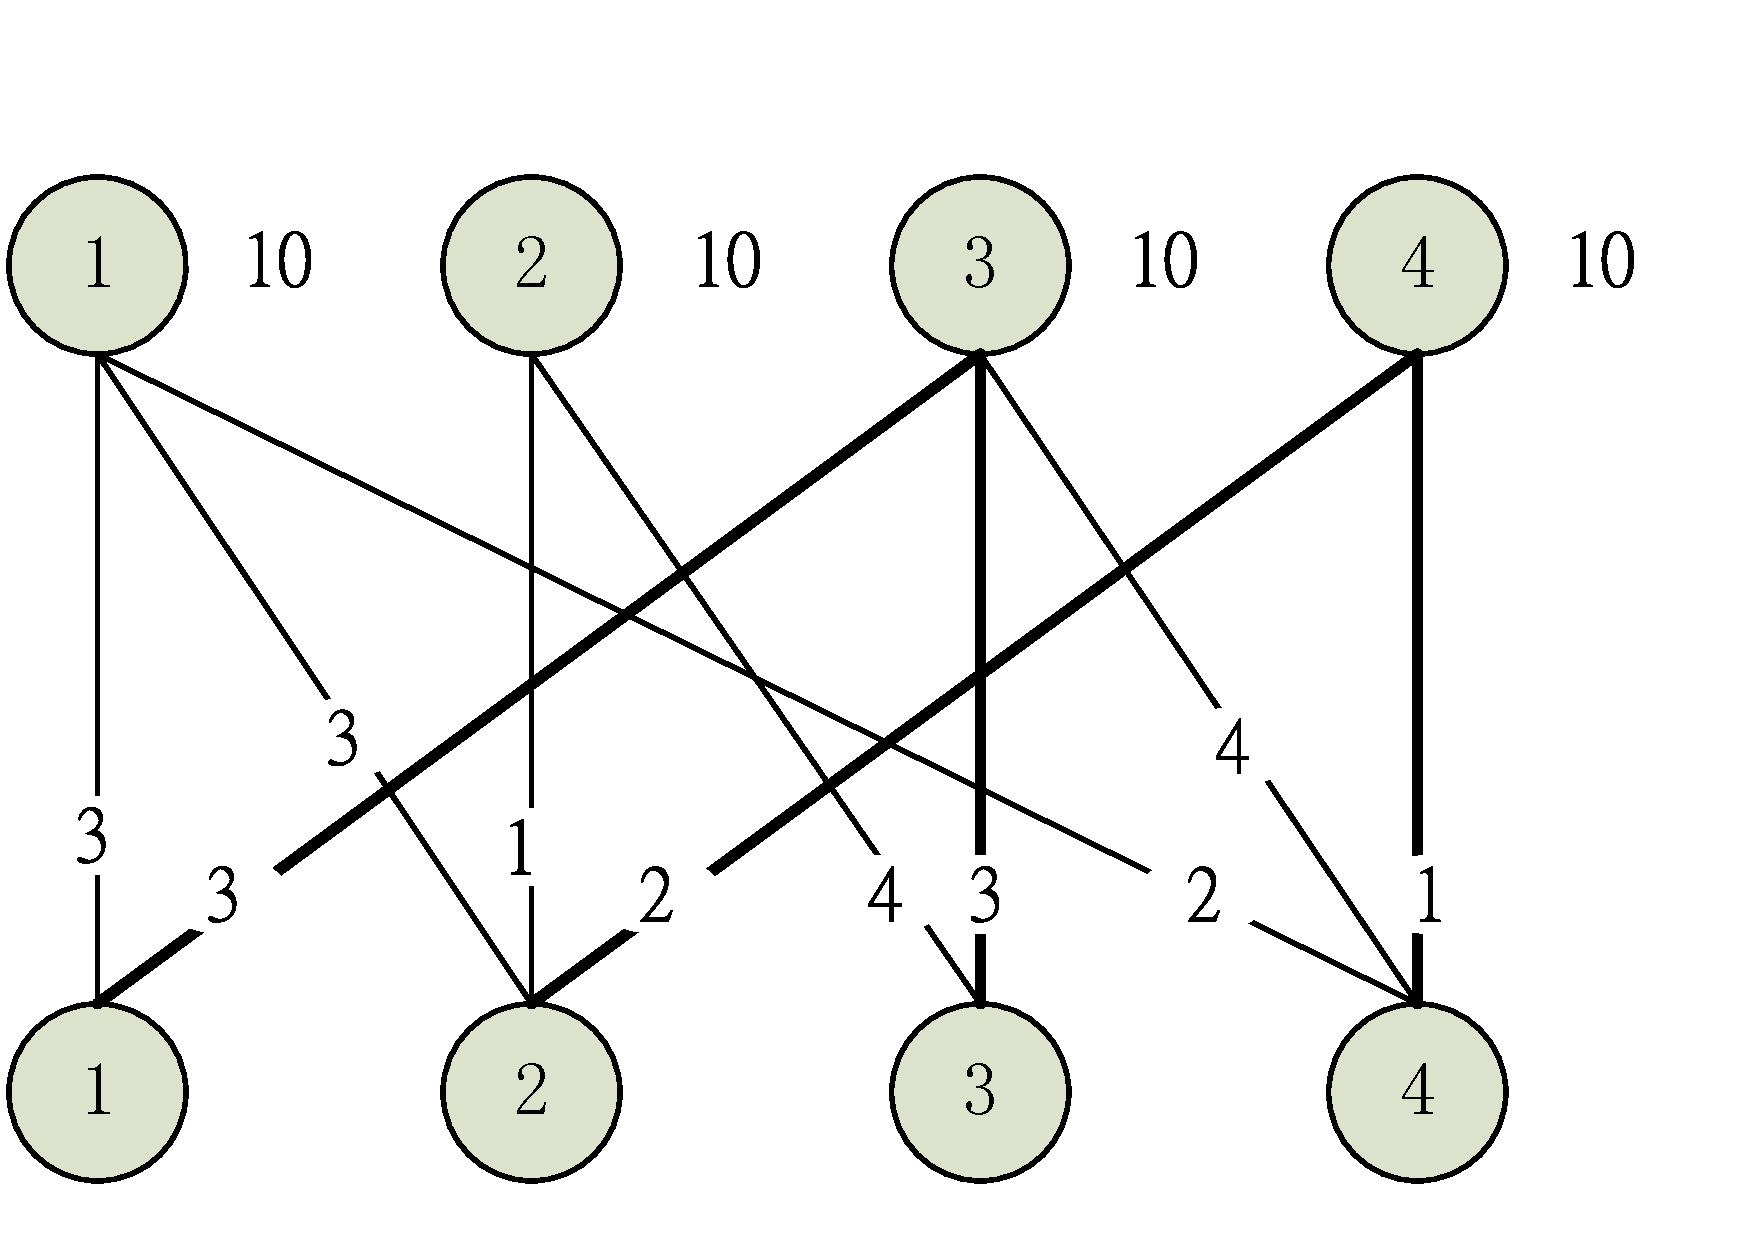
\includegraphics[width=0.5\textwidth]{figure-1.pdf}
\caption{\label{figure:exampleUFL}An example of a UFL game}
\vspace{-3mm}
\end{figure}

In the UFL game shown in Figure \ref{figure:exampleUFL}, there are four facilities and four customers (players). Each facility has a fixed opening cost 10. The numbers on the links are the transportation costs from facilities to customers. An optimal decision for the grand coalition is to open facilities 3 and 4, and the links in bold are the optimal paths. Therefore, the grand coalition cost is 10+10+3+3+2+1=29.

For this example, we use two LP solvers, the ``Simplex" and ``Interior Point" methods, in MATLAB Release 2011a to compute the LPB allocations, respectively.
Table \ref{table:UFLCA} shows the cost assigned to each player under different approaches.

\begin{table}[H]
\vspace{-2mm}
\centering
\tabcolsep=4pt
\small
\renewcommand\arraystretch{1.5}
\caption{\label{table:UFLCA} Optimal stable UFL cost allocations under different approaches}
\vglue5pt
\begin{tabular}[!h]{c c c c c c c c c c c c c}
\hline
\multicolumn{1}{c}{Method} &\multicolumn{1}{c}{} &\multicolumn{1}{c}{Player 1} &\multicolumn{1}{c}{} &\multicolumn{1}{c}{Player 2} &\multicolumn{1}{c}{} &\multicolumn{1}{c}{Player 3} &\multicolumn{1}{c}{} &\multicolumn{1}{c}{Player 4}	&\multicolumn{1}{c}{} &\multicolumn{1}{c}{Total Shared Cost}\\
\hline
LPB with Simplex	& &5.00	& &6.50	& &8.50	& &6.50	&	&26.5	&\\
LPB with Interior Point	& &6.58	& &6.50	& &8.50	& &4.92	&	&26.5	&\\
LRB	& &6.87	& &6.50	& &8.50	& &4.63	&	&26.5	&\\
\hline
\end{tabular}
\vspace{-3mm}
\end{table}


The example reveals that the LRB algorithm can generate optimal stable cost allocations that are different from those generated by common LP solvers.
The LRB solution is beyond the range of convex combination of the two LPB solutions.
This demonstrates the value of the LRB algorithm in providing alternative cost allocations.


To investigate the capability of the LRB algorithm under a general setting, we tested 30 uncapacitated facility location benchmark instances developed by \cite{Benchmark}, all with $m=n=100$. We conducted all computational experiments  on a Windows 7 PC with an Intel Core i7-2600 running at 3.4GHz and 16G RAM. All algorithms were implemented in MATLAB Release 2011a.
Among the 30 instances there are 22 for which the LRB solution is  beyond the range of convex combination of the two LPB solutions.
Again, this shows the value of the LRB algorithm in terms of computationally finding alternative optimal stable cost allocations even in cases where the LPB cost allocations are shown to be optimal.
